%
% Simple asymmetric two-column CV 
% Author: Sofia JIJON
%

\documentclass[a4paper,10pt]{article}
\usepackage[vmargin=1.5cm, hmargin=1.2cm]{geometry}
% !TEX root = Simple-CV.tex
%-------------------------------------------------------------------------------------------------------
% Packages
%-------------------------------------------------------------------------------------------------------
\usepackage[english]{babel}
\usepackage[utf8]{inputenc}
\usepackage{fontawesome}
\usepackage{datetime}
\usepackage[usenames,dvipsnames]{xcolor}
\usepackage[colorlinks=true, urlcolor=ColorTwo]{hyperref}
\usepackage{tikz}
\usepackage{hyperref}
\usepackage{setspace}
\usepackage{graphicx}
\usepackage{enumitem}
\usepackage{sectsty}
\usepackage{multicol}
\usepackage{adjustbox}
%-------------------------------------------------------------------------------------------------------
% Layout
%-------------------------------------------------------------------------------------------------------
\pagenumbering{gobble}
\renewcommand{\baselinestretch}{1.5} 
\setlength{\parindent}{0pt}

%
% Color theme
%
\definecolor{ColorOne}{RGB}{0,0,0} 	% Blue
\definecolor{ColorTwo}{RGB}{106,106,106} 	% Mauve
%\definecolor{ColorTwo}{RGB}{140,100,0} 	% Gold

\sectionfont{\color{ColorOne}} 
\subsectionfont{\color{ColorOne}} 

%
% Vertical line
%
\newcommand{\MyVerticalRule}{%
	\textcolor{ColorOne}{\rule{1pt}{\textheight}}
}

%
% Update
%
\newcommand{\LastUpdate}{%
\vfill
\centering \small
\textcolor{ColorOne}{Last updated: \monthname,~\the\year }
}

%
% Skip
%
\newcommand{\MySkip}{
\vskip12pt
}

%
% Format hyperrefs
%
\newcommand{\myhref}[2]{%
\href{#1}{\textcolor{ColorTwo}{#2}}
}
%
% Format skill bullets
%
\newcommand{\SkillBull}[1]{%
\textcolor{ColorTwo}{#1}
}


%-------------------------------------------------------------------------------------------------------

\begin{document}
\thispagestyle{empty}

%-------------------------------------------------------------------------------------------------------
% Left column
%-------------------------------------------------------------------------------------------------------
\begin{adjustbox}{valign=t}
\begin{minipage}{0.3\textwidth} % Adapt width to your convenience
%----------------------------------------------------
% Please add a photo in 1x1 format
\begin{center}
\begin{tikzpicture}
	\clip (0,0) circle (2cm) node {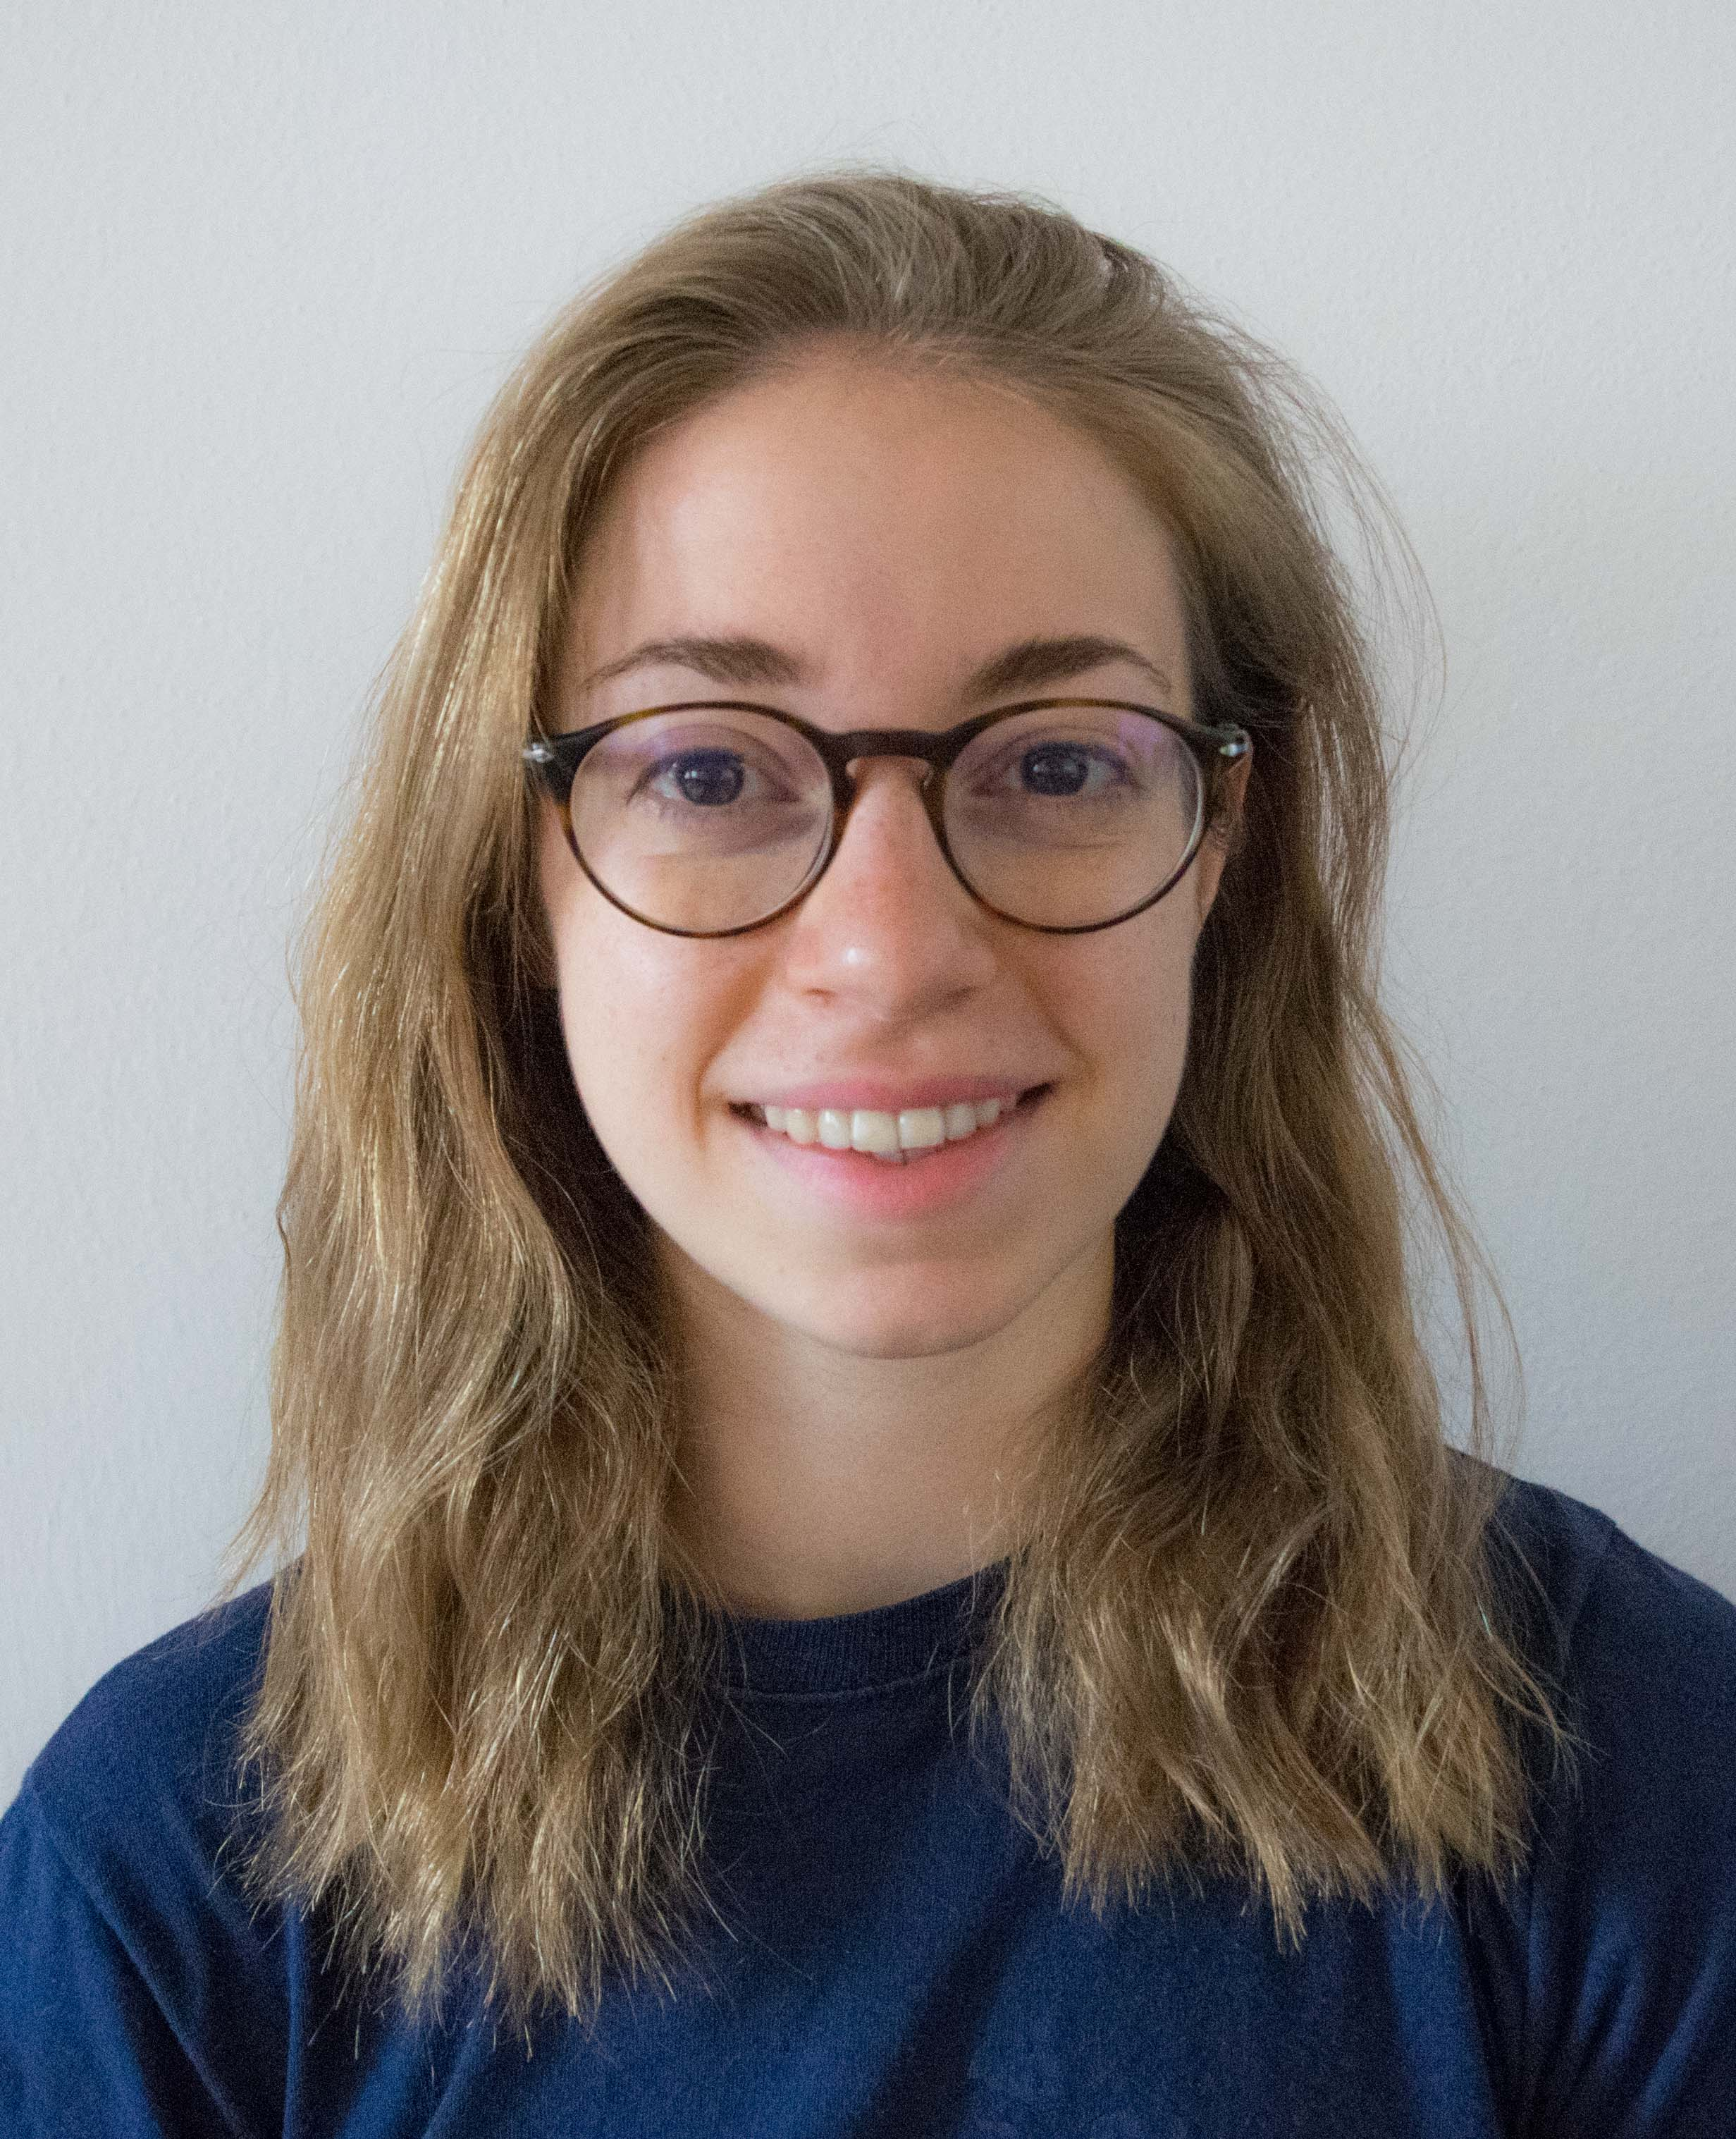
\includegraphics[width=4cm]{propic}};
\end{tikzpicture}

\MySkip 	% See MySetup.tex file

%----------------------------------------------------
{\LARGE \bfseries Elena Acinapura}

\MySkip 	% See MySetup.tex file

Born in Bolzano, Italy, 1999
Currently living in Zürich\\

\MySkip 	% See MySetup.tex file

\textcolor{ColorTwo}{\faEnvelopeO} 
\myhref{mailto:elena.acinapura@gmail.com}{elena.acinapura@gmail.com} \\

\textcolor{ColorTwo}{\faChain} 
\myhref{https://elena.acinapura.it}{elena.acinapura.it}
\end{center}

\vfill

%----------------------------------------------------
\section*{Scientific interests}
\raggedright
\textcolor{ColorOne}{$\circ$} Quantum computing\\
\textcolor{ColorOne}{$\circ$} Quantum sensing\\
\textcolor{ColorOne}{$\circ$} Computational physics\\

\vfill

%----------------------------------------------------
\section*{Education}
	\begin{description}
	\raggedright
	\item [\normalfont \textcolor{ColorTwo}{2021 - Now}]
    \textbf{Master in Quantum Engineering}\\
	ETH Zürich\\
	Zürich -- Switzerland

	\item [\normalfont \textcolor{ColorTwo}{2018 - 2021}] \textbf{Bachelor in
	Physics}\\
	University of Trento\\
	Trento -- Italy\\
    \small{Graduated with 110/110 cum laude}
    \normalsize

	\item [\normalfont \textcolor{ColorTwo}{2013 - 2018}] \textbf{Secondary School}\\ 
	Liceo Classico \textit{"G. Carducci"} \\
	Bolzano -- Italy \\
    \small{Concluded with 100/100 cum laude} \normalsize
\end{description}

\vfill
\end{minipage}
\end{adjustbox}
%
%
%-------------------------------------------------------------------------------------------------------
% Vertical rule
%-------------------------------------------------------------------------------------------------------
%
\hfill
\begin{adjustbox}{valign=t}
\begin{minipage}{0.05\textwidth} % Adapt width to your convenience
\MyVerticalRule  % See MySetup.tex file
\end{minipage}
\end{adjustbox}
\hfill
%
%-------------------------------------------------------------------------------------------------------
% Right column
%-------------------------------------------------------------------------------------------------------
\begin{adjustbox}{valign=t}
\begin{minipage}{0.6\textwidth} % Adapt width to your convienience

%----------------------------------------------------
\section*{Working Experience}
\begin{description}
\raggedright
\item[\normalfont \textcolor{ColorTwo}{Jul. 2021 -- Dec. 2021.}] 
	\textbf{Technical consultant}\\
	
	\emph{Kerr Italy s.r.l.}\\
	\small
	Development of the front-end electronics for a single-photon detector.
	\normalsize
\item[\normalfont \textcolor{ColorTwo}{Feb. 2021 -- Jun. 2021}] 
	\textbf{Physics Tutor}\\
	
	\emph{University of Trento}\\
	\small 
	Tutor for the Physics course at the department of Industrial Engineering
    \normalsize
\end{description}
%----------------------------------------------------
\section*{Technical Skills}
\begin{description}
\item \textbf{C/C++} --\small  Solid knowledge; used extensively for computational physics and algorithms. Ability of building and linking complex libraries. \normalsize
\item \textbf{Python} --\small Very good knowledge; used extensively for scientific analysis and personal projects.\normalsize
\item \textbf{Git} --\small Extensive and every-day use of Git for version control of personal and shared projects.\normalsize
\item \textbf{CMake} -- \small Discrete skills in building structured project in C/C++. Used in scientific and personal projects.\normalsize
\item \textbf{System Verilog, FPGA programming} -- \small Knowledge gained following the VLSI I course at ETH Zürich.\normalsize
\item \LaTeX -- \small Very good knowledge, used extensively.\normalsize
\item \textbf{Linux} -- \small Long-time Linux user.\normalsize
\end{description}
\small 
Furthermore, I have a good knowledge of written and spoken English and a discrete knowledge of German.
\normalsize
%----------------------------------------------------
\section*{Further Experiences}
\begin{description}
\raggedright
\item[\normalfont \textcolor{ColorTwo}{March 2021}] 
	\textbf{SWERC Competition}\\
	\small
	I participated in SWERC, the international university competition of competitive programming, as a student selected from the University of Trento.
	\normalsize
\item[\normalfont \textcolor{ColorTwo}{Nov 2020 - Jul 2021}] 
	\textbf{Member of the Department Council}\\
	
	\emph{University of Trento}\\
	\small 
	I have been elected member of the Physics Department Council at Trento University, in representation of the physics students.
    \normalsize
\end{description}

\MySkip
\LastUpdate
\end{minipage}
\end{adjustbox}
\end{document}